
\subsection{Analyse VBB Verkehrsverbund Berlin-Brandenburg GmbH}
In der Kategorie der Personenbeförderung wurde die Webseite des VBB Verkehrsverbund Berlin-Brandenburg GmbH ausgewählt.

Ein Fehler der auf der Website wiederholt auftritt, ist der Verstoß gegen Kriterium 1.4.3 "Mindestkontrast". Dabei handelt es sich um Kontrastprobleme zwischen Text und Hintergrund. Betroffen sind davon die Texte im Menü, einige Überschriften und Stichpunkte und Buttons auf der Startseite.

\begin{figure}[H]
    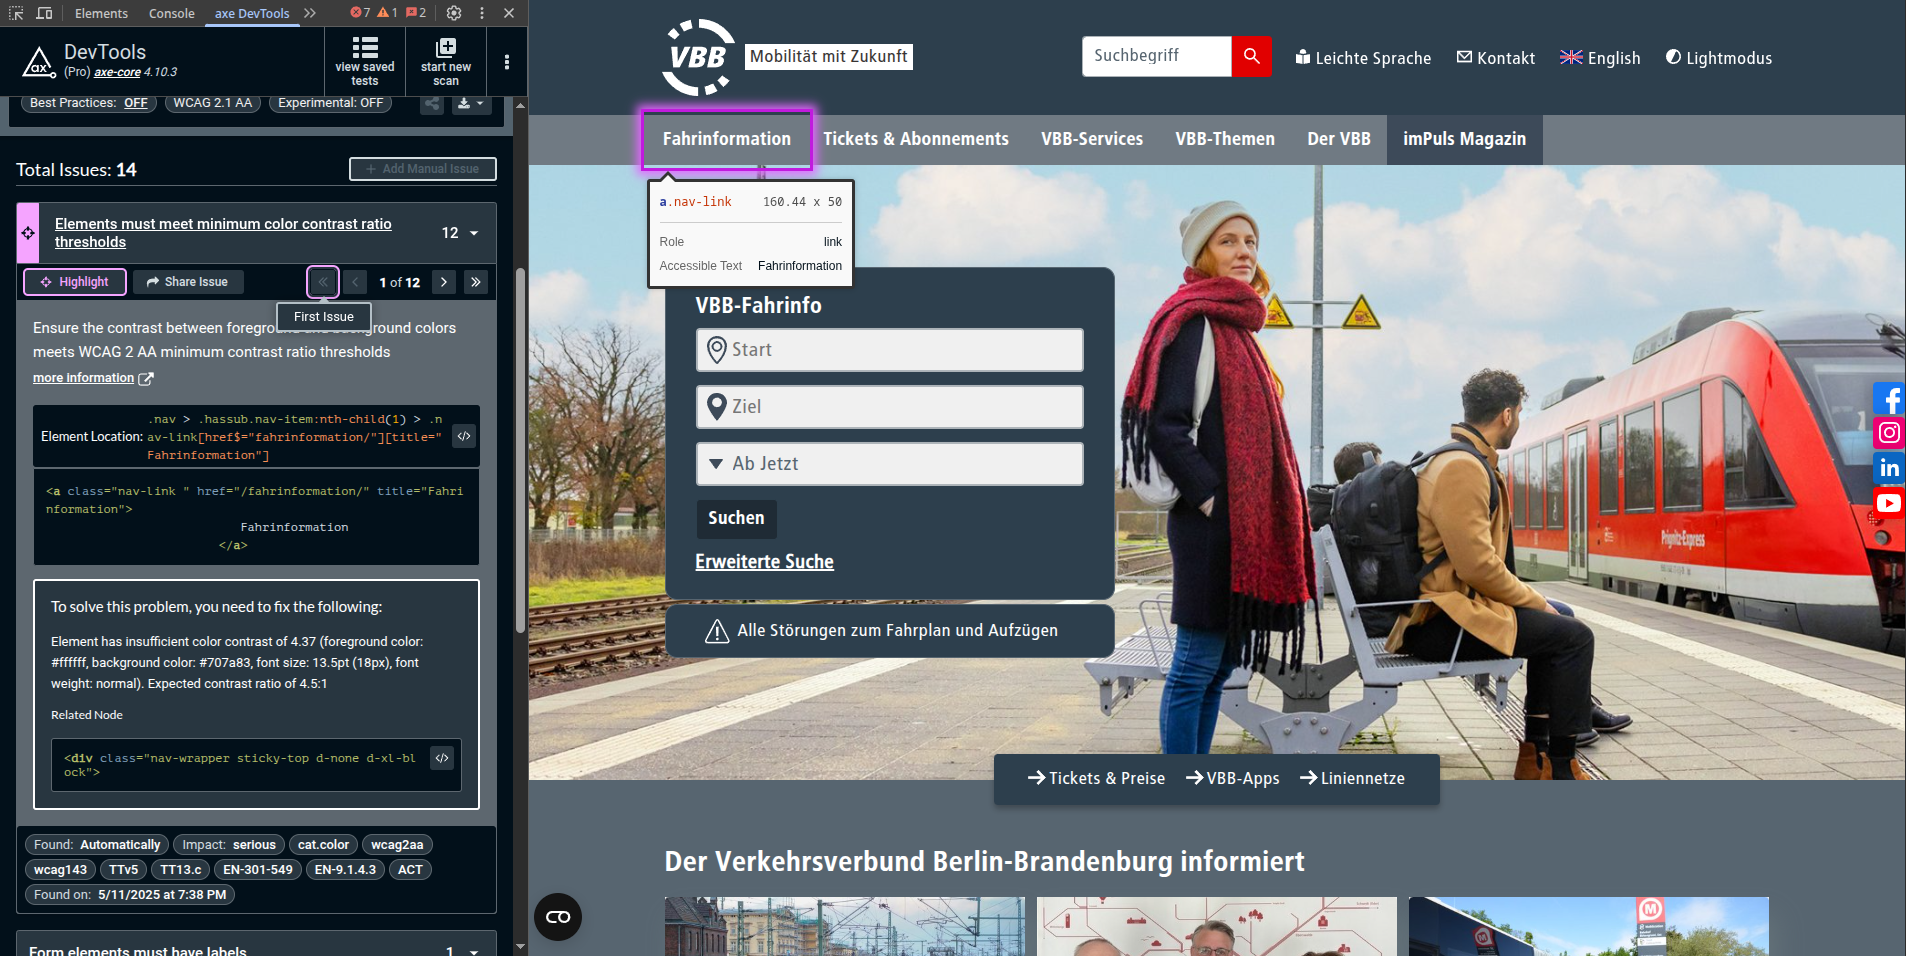
\includegraphics[width=\textwidth]{img/vbb_failed-minimum-contrast.png}
    \caption{Kontrastprobleme auf der Startseite}
\end{figure}

Außerdem fehlen auch hier, wie bei der Sparkasse auch, Labels bei den Suchfeldern. Dies Verstößt gegen 4 WCAG-Kriterien 1.1.1 "Nicht-Text-Inhalt", 1.3.1 "Info und Beziehungen", 2.4.6 "Überschriften und Beschriftungen" und 3.3.2 "Labels oder Anleitungen". 

\begin{figure}[H]
    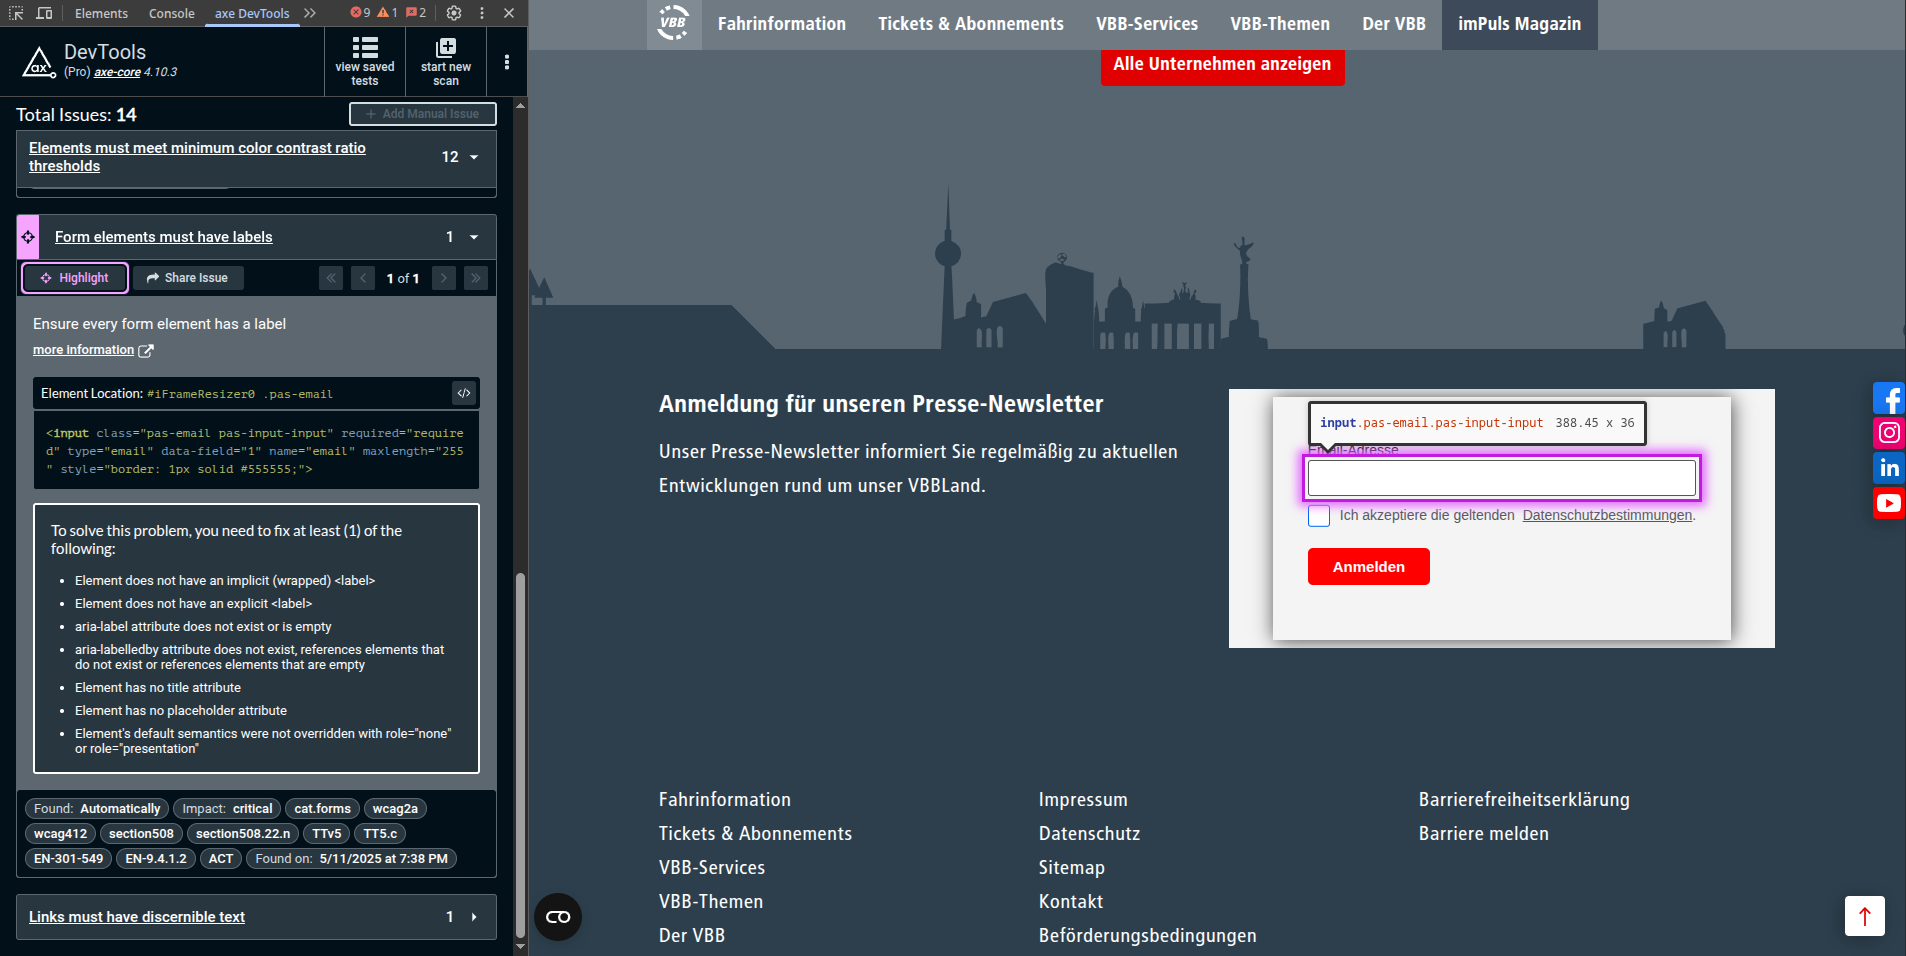
\includegraphics[width=\textwidth]{img/vbb_no-label.png}
    \caption{Fehlendes Label bei einem Suchfeld}
\end{figure}

Weitere Grundlegende Elemente wie alternative Texte für Bilder fehlen auch auf dieser Seite. Diese sind wichtig um den Inhalt der Seite auch für Screenreader und Maschinen lesbar zu machen. 

\begin{figure}[H]
    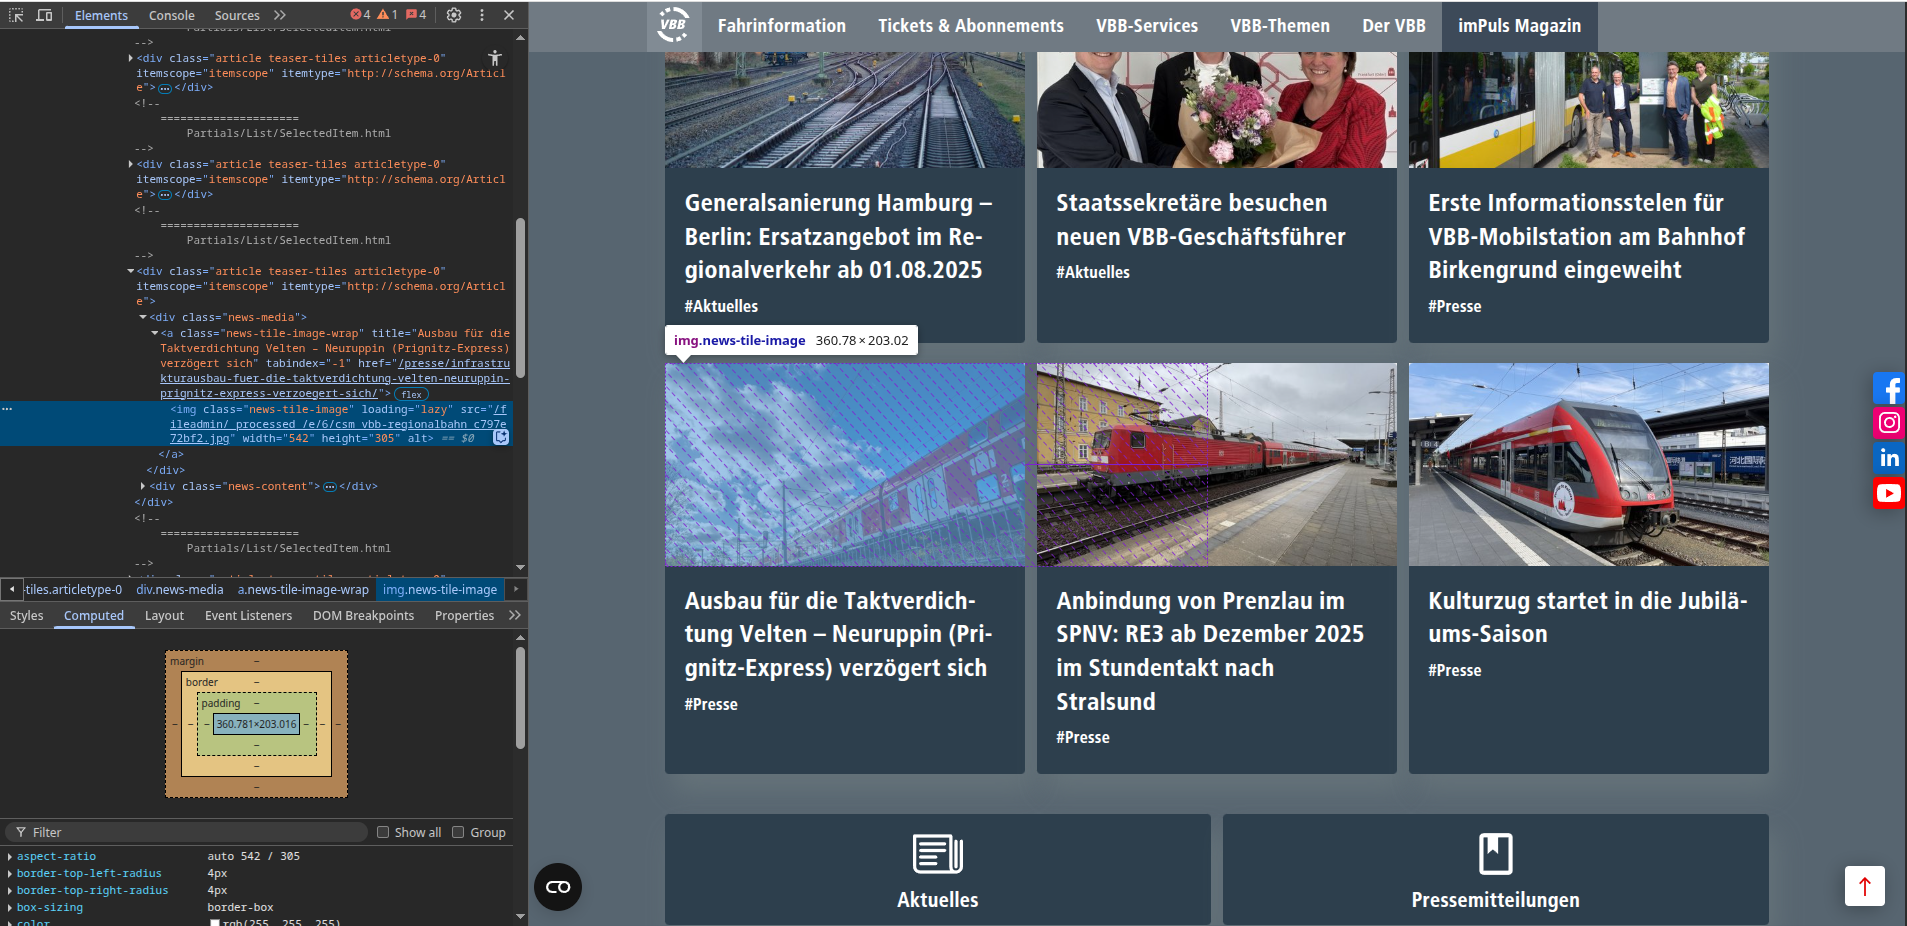
\includegraphics[width=\textwidth]{img/vbb_no-alt-text.png}
    \caption{Fehlender alternativer Text}
\end{figure}

Durch die hablautomatisierten Tests ist ein weiterer gravierender Mangel festgestellt worden. Die Startseite ist nicht vollständig mit der Tastatur bedienbar. Die Seite enthält einen Slider, der die Logos der Verkehrsunternehmen anzeigt. Dieser Slider fängt wieder von vorne an, wenn man das Ende erreicht. Das passiert aber auch, wenn man mit der Tastatur navigiert und im Slider hängen bleibt. Man ist also in einer sogenannten Keyboard-Trap gefangen und kann nicht mehr vorwärts oder rückwärts navigieren. Das angesprochene Element ist in Abbildung 4.11 zu sehen.

\begin{figure}[H]
    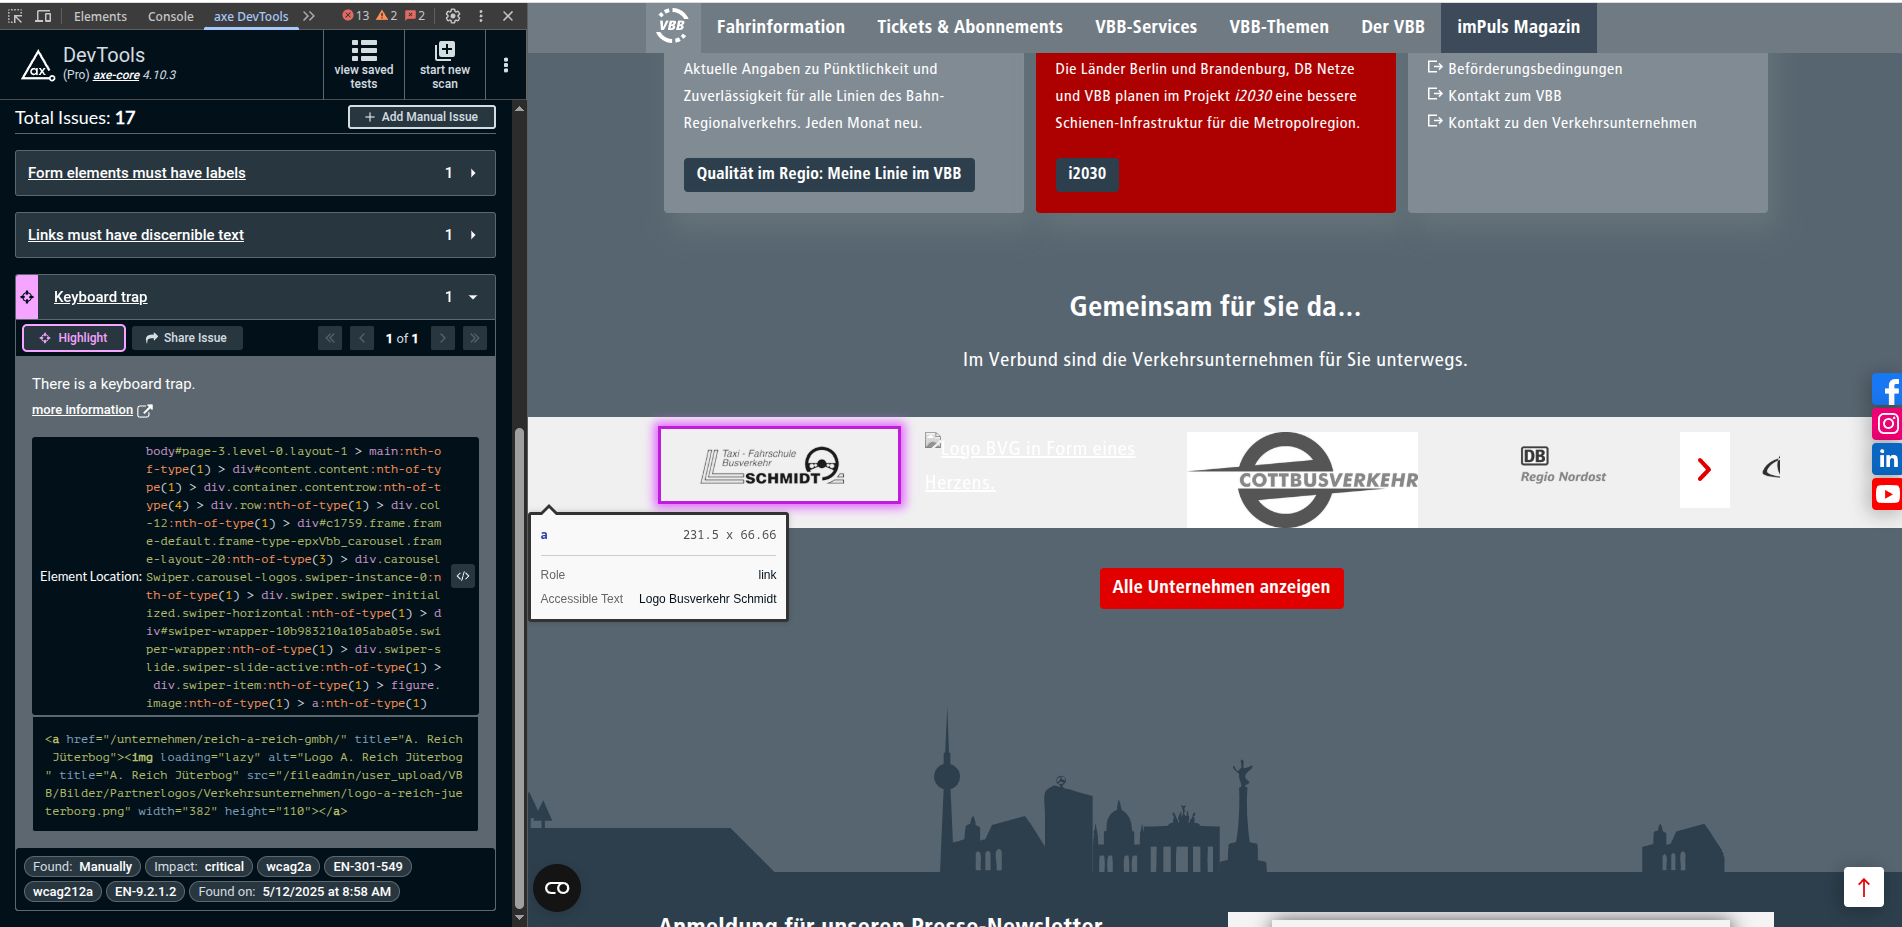
\includegraphics[width=\textwidth]{img/vbb_keyboard-trap.png}
    \caption{Slider mit Keyboard-Trap}
\end{figure}

Im Bereich der Tastaturbedienbarkeit sind auch einige Elemente nicht korrekt fokussierbar. Wenn die Seite manuell mit der Tastatur bedient wird, verschwindet der Fokus für 2 Tabstops. Damit ist das Kriterium 2.4.7 "Fokussierbarkeit" nicht erfüllt.

Auf den Unterseitenm, wie die Fahrinfo, wiederholen sich die Kontrastfehler, da das Menü konstant auf den verschiedenen Seiten angelegt ist. Allerdings hat der iframe keinen zugänglichen Namen. Dies ist ein Verstoß gegen Kriterium 4.1.2 "Name, Rolle, Wert".

\begin{figure}[H]
    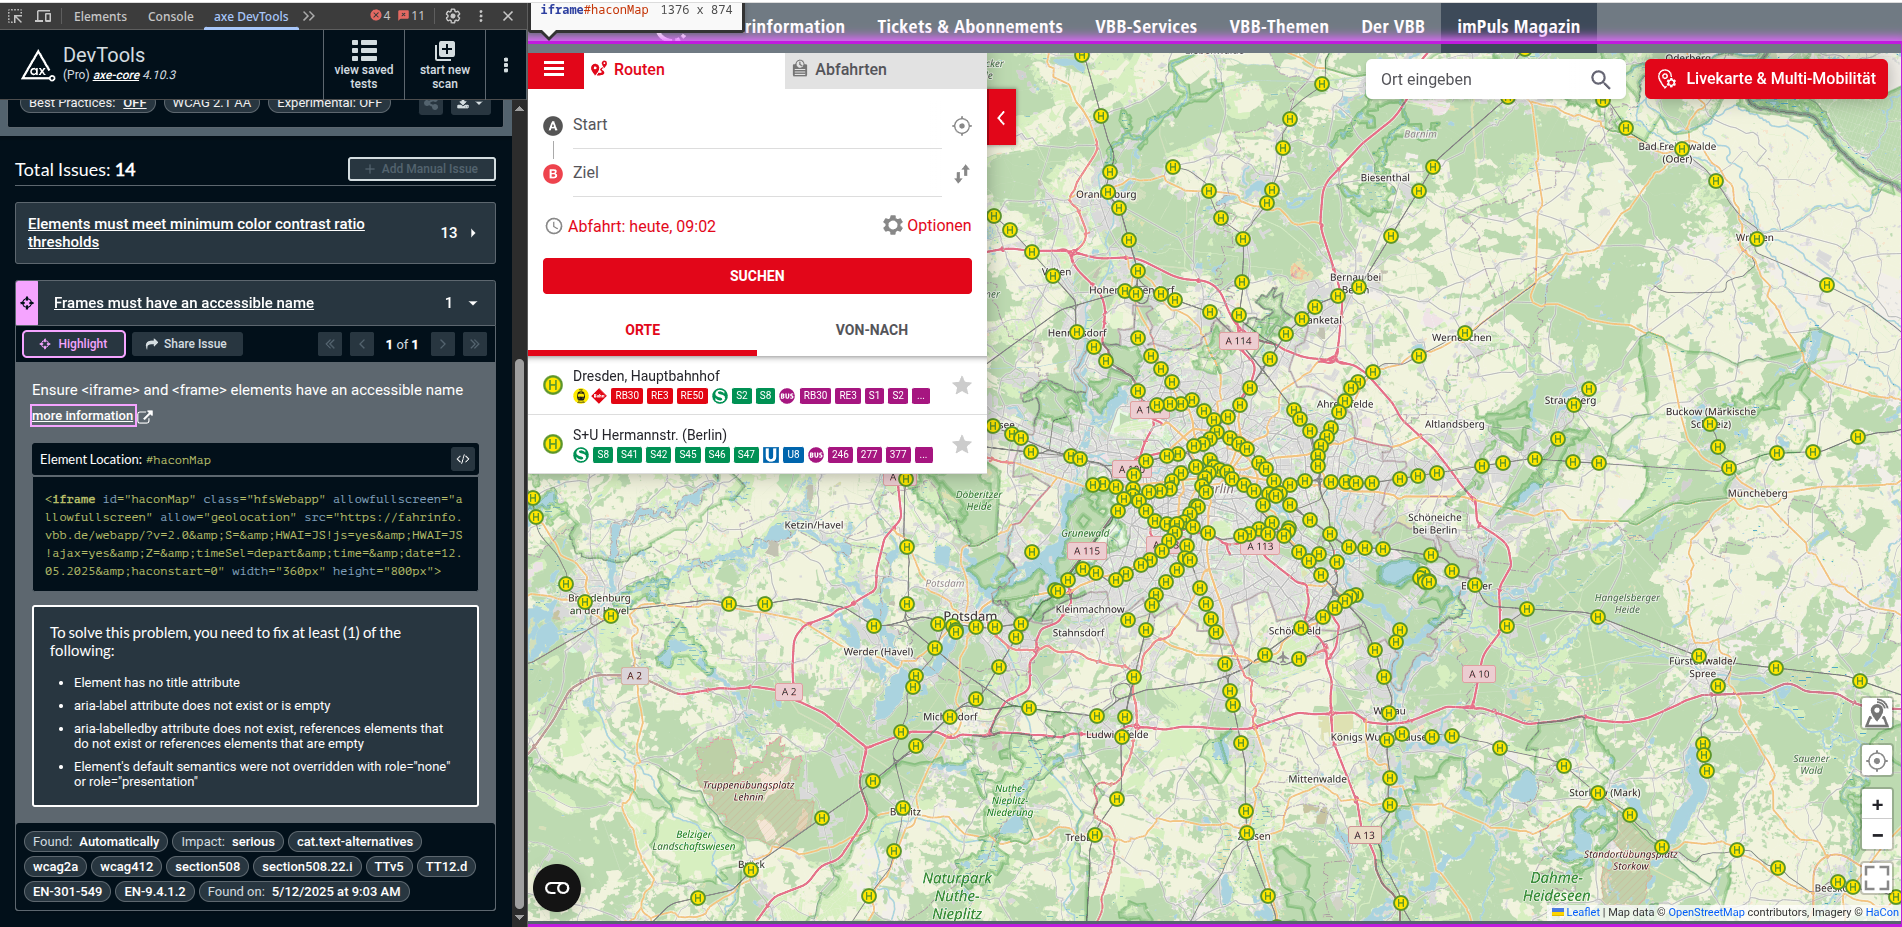
\includegraphics[width=\textwidth]{img/vbb_no-frame-name.png}
    \caption{Iframe ohne zugänglichen Namen}
\end{figure}

Insgesamt treten auf der Seite deutlich mehr Fehler auf als bei den vorherigen Seiten. Auch hier überscheiden sich wieder einige Fehler. Es sind aber auch neue Fehler aufgetreten, vor allem im Bereich der Tastaturbedienbarkeit.

\begin{figure}[H]
\begin{tikzpicture}
\begin{axis}[
    width=\textwidth,
    height=10cm,
    ybar,
    bar width=12pt,
    xlabel={WCAG-Kriterium},
    ylabel={Fehleranzahl},
    symbolic x coords={ 9.1.1.1, 9.1.4.3, 9.2.1.1, 9.2.4.4, 9.2.4.7, 9.4.1.2 },
    xtick=data,
    x tick label style={rotate=45, anchor=east},
    ymin=0,
    ymax=300,
    enlarge x limits=0.1,
    legend style={cells={anchor=west}, legend pos=north east},
    nodes near coords,
    nodes near coords style={font=\scriptsize},
]
\addplot table[x=WCAG-Kriterium,y=Fehleranzahl_axe,col sep=tab] {csv/output/wcag_analyse_vbb_xxxx.csv};
\addplot table[x=WCAG-Kriterium,y=Fehleranzahl_WAVE,col sep=tab] {csv/output/wcag_analyse_vbb_xxxx.csv};
\legend{axe,WAVE}
\end{axis}
\end{tikzpicture}
\caption{Auswertung Analyse VBB}
\end{figure}